% !TeX program = xelatex
\documentclass{article}
\usepackage[fontset=fandol]{ctex}
\usepackage{titlesec,hyperref,tikz}
\usetikzlibrary{datavisualization}
\titleformat{\section}[hang]{\Large\bfseries}{第\thesection 节}{1em}{}
\titlespacing*{\section}{0pt}{12pt}{6pt}
\renewcommand{\sectionautorefname}{节}
\begin{document}
\section{包定义的标题}\label{sec:layout}
即时预览读取标题格式与中文图表名称。
这里有一个显式换行。\newline 第二行仍然可以编辑。
\begin{table}[ht]
\centering
\begin{tabular}{cc}名称&数值\\甲&1\\乙&2\end{tabular}
\caption{中文表题}\label{tab:layout}
\end{table}\newline
表格后换行不会使预览失败。

\begin{figure}[ht]
\centering
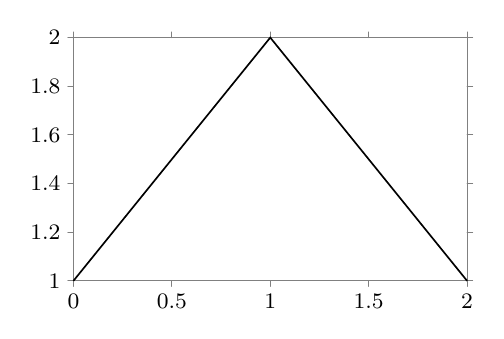
\begin{tikzpicture}
\datavisualization [scientific axes, visualize as line]
data {x,y
0,1
1,2
2,1
};
\end{tikzpicture}
\caption{中文图题}\label{fig:layout}
\end{figure}
TikZ 环境可以显示图形预览，也可展开灰色源码框编辑；永久预览由 \TeX{} 编译。

\autoref{sec:layout}、图~\ref{fig:layout} 和表~\ref{tab:layout} 使用源码中的标签。
\end{document}
